\section{Verteilungssicht}
Jeder Microservice wird als eigener Docker-Container betrieben. Die Container kommunizieren über Service-Namen im gemeinsamen Docker-Compose-Netzwerk. Dadurch müssen keine IP-Adressen im Source Code fest verdrahtet werden.

\begin{tabularx}{\textwidth}{L{6.8cm}L{2.0cm}Y}
\toprule
\textbf{Container} & \textbf{Port} & \textbf{Zustand} \\
\midrule
\makecell[l]{configuration-service} & 8081 & persistentes eigenes Volume \\
\makecell[l]{analysis-management-service} & 8082 & persistentes eigenes Volume \\
\makecell[l]{fluid-analysis-service} & 8083 & stateless \\
\makecell[l]{thermal-analysis-service} & 8084 & stateless \\
\makecell[l]{electrical-analysis-service} & 8085 & stateless \\
\makecell[l]{engine-management-analysis-service} & 8086 & stateless \\
\bottomrule
\end{tabularx}

\begin{figure}[h]
  \centering
  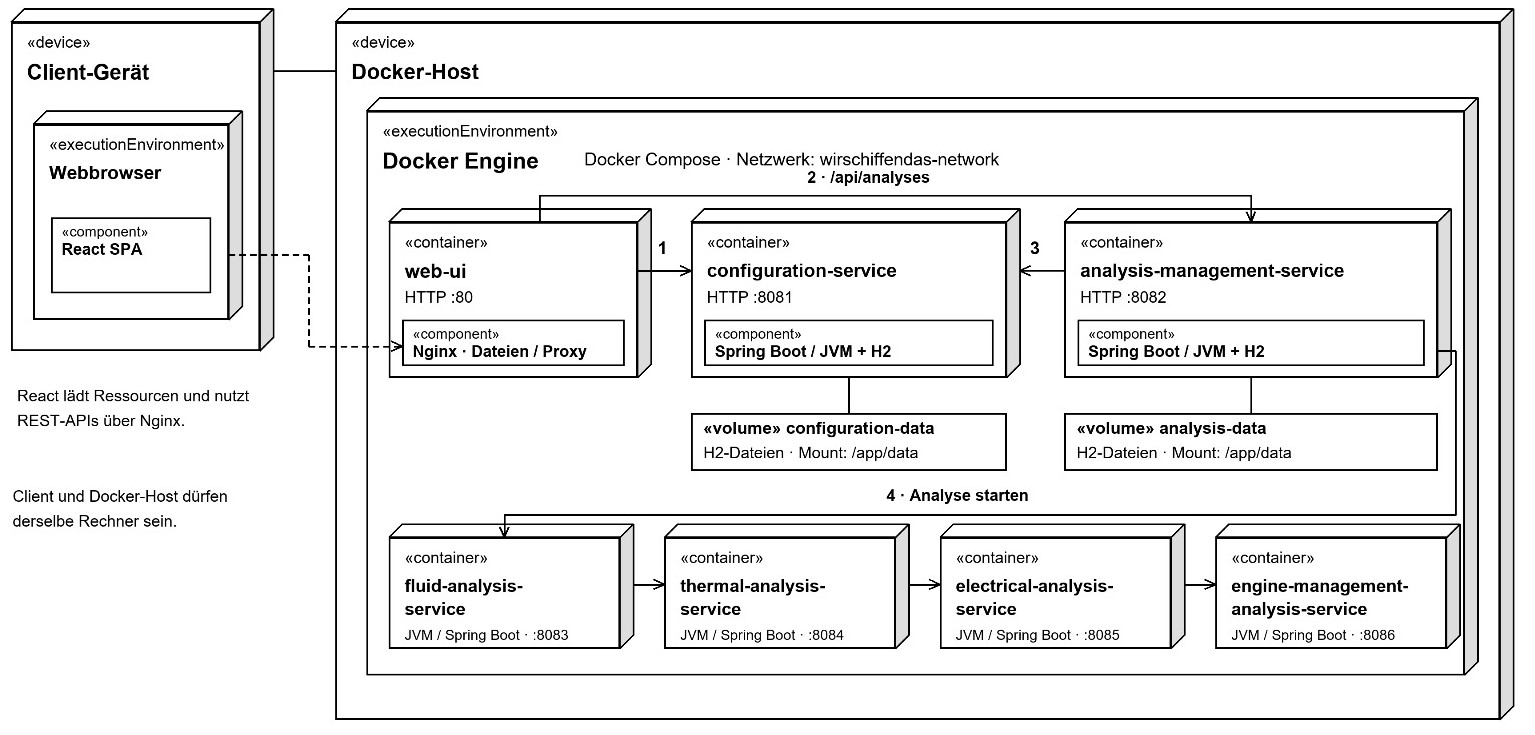
\includegraphics[width=\textwidth]{../diagrams/Verteilungssicht.jpeg}
  \caption{Verteilungssicht: Container, Ports und Docker-Compose-Netzwerk.}
\end{figure}

\subsection{Deployment-Prinzipien}
\begin{itemize}
  \item Eigener Container pro Microservice.
  \item Getrennte Persistenz für Configuration Management und Analysis Management.
  \item Stateless Analyse-Services für einfacheres unabhängiges Starten, Stoppen und Skalieren.
  \item Compose-DNS statt fest verdrahteter IP-Adressen.
  \item Zwei Varianten im Repository: veröffentlichte Images und lokaler Build aus dem Source Code.
\end{itemize}

\newpage

\section{Querschnittliche Konzepte}
\subsection{Status- und Ergebnismodell}

Resultate sind \code{OK} oder \code{FAILED}. Das Overall Result bleibt offen, solange noch Schritte ausstehen. Es wird \code{FAILED}, sobald ein relevanter Algorithmus fehlschlägt, und \code{OK}, sobald alle vier Algorithmen erfolgreich abgeschlossen sind.

\vspace{1cm}
\begin{center}
\begin{tikzpicture}[
  node distance=12mm,
  every node/.style={font=\small},
  state/.style={draw=darkblue,rounded corners,fill=lightblue,minimum width=30mm,minimum height=10mm,align=center},
  failed/.style={draw=warnorange,rounded corners,fill=warnorange!10,minimum width=30mm,minimum height=10mm,align=center}
]
\node[state] (p) {PENDING};
\node[state,right=of p] (r) {RUNNING};
\node[state,right=of r] (ready) {READY};
\node[failed,below=of r] (f) {FAILED};
\draw[-{Latex},thick] (p) -- (r);
\draw[-{Latex},thick] (r) -- (ready);
\draw[-{Latex},thick] (r) -- (f);
\end{tikzpicture}
\end{center}
\vspace{0.5cm}

\subsection{Resilience}
Resilience4j implementiert den Circuit Breaker für ausgehende Aufrufe zwischen Services \cite{richardson2018patterns}. Das Zustandsmodell folgt \emph{Closed -- Open -- Half-Open}. Im normalen Zustand werden Aufrufe zugelassen. Nach ausreichenden Fehlern öffnet der Breaker und blockiert weitere Aufrufe. Nach einer Wartezeit werden begrenzte Testaufrufe zugelassen.

\subsection{Persistenz und Datenhoheit}
Nur Configuration Management und Analysis Management besitzen langfristigen Zustand. Die Analyse-Services sind bewusst stateless. Damit bleiben fachliche Datenhoheit und Bounded-Context-Grenzen klar erkennbar.

\newpage

\section{Architekturentscheidungen}
\subsection{ADR-01: Fachlicher Schnitt statt technischer Layer}
\textbf{Entscheidung:} Die Microservices werden nach Business Capabilities getrennt.\\
\textbf{Begründung:} Fachliche Verantwortung, Datenhoheit und Deployment-Einheit bleiben zusammen. Dies reduziert das Risiko eines \emph{Wrong Cut}.

\subsection{ADR-02: REST/HTTP für Version 1}
\textbf{Entscheidung:} Der PoC verwendet REST/HTTP für die Service-Kommunikation.\\
\textbf{Begründung:} Die Kommunikation ist leicht nachvollziehbar, demonstrierbar und testbar. Der Trade-off ist eine stärkere temporale Kopplung als bei asynchronem Messaging.

\subsection{ADR-03: Choreographie statt zentraler Orchestration}
\textbf{Entscheidung:} Analysis Management startet nur den Anchor-Schritt. Danach gibt jeder erfolgreiche Analyse-Service die Verarbeitung weiter.\\
\textbf{Begründung:} Die geforderte Zusammenarbeit der Analysealgorithmen bleibt dezentral sichtbar.

\subsection{ADR-04: Circuit Breaker mit Resilience4j}
\textbf{Entscheidung:} Service-zu-Service-Aufrufe werden mit Circuit Breakern geschützt.\\
\textbf{Begründung:} Der Ausfall eines Analyse-Services wird lokal begrenzt und als kontrollierter Zustand sichtbar.

\subsection{ADR-05: Container pro Microservice}
\textbf{Entscheidung:} Jeder Service besitzt ein eigenes Dockerfile und einen eigenen Container.\\
\textbf{Begründung:} Dies unterstützt Independent Deployability und erfüllt die technische Semesterprojektanforderung zu Docker/Docker Compose.

\subsection{ADR-06: Keine Shared Persistence}
\textbf{Entscheidung:} Configuration Management und Analysis Management besitzen getrennte Daten. Analyse-Services bleiben stateless.\\
\textbf{Begründung:} Die Kopplung zwischen Bounded Contexts wird reduziert; eine gemeinsame Datenbank wird nicht als Integrationsmechanismus verwendet.

\newpage

\section{Qualitätsanforderungen und Architecture Smells}
\subsection{Priorisierte Probleme und Gegenma\ss{}nahmen}
\begin{tabularx}{\textwidth}{L{1.2cm}L{5.0cm}Y}
\toprule
\textbf{Prio} & \textbf{Smell / Anti-Pattern} & \textbf{Behandlung im Proof-of-Concept} \\
\midrule
1 & Isolation of Failures & Circuit Breaker, kontrollierter Fehlerzustand und gezielter Retry. \\
2 & Independent Deployability & Eigener Build und eigener Docker-Container pro Service. \\
3 & Wrong Cut & DDD-basierte Zerlegung nach fachlichen Fähigkeiten statt nach technischen Layern. \\
4 & Shared Persistence & Getrennte Datenhoheit und DTO-basierte Integration. \\
\bottomrule
\end{tabularx}

Zusätzlich adressiert die Architektur \emph{Hard-Coded Endpoints} durch Compose-DNS und verbessert \emph{Insufficient Monitoring} durch ein explizites Statusmodell und die UI-Sicht auf laufende Analysen. Für einen produktiven Betrieb bleiben zentralisiertes Logging, verteiltes Tracing, Authentisierung/Autorisierung, API-Versionierung und ein dedizierter Observability-Stack als Ausbaustufen offen.

\begin{figure}[h]
  \centering
  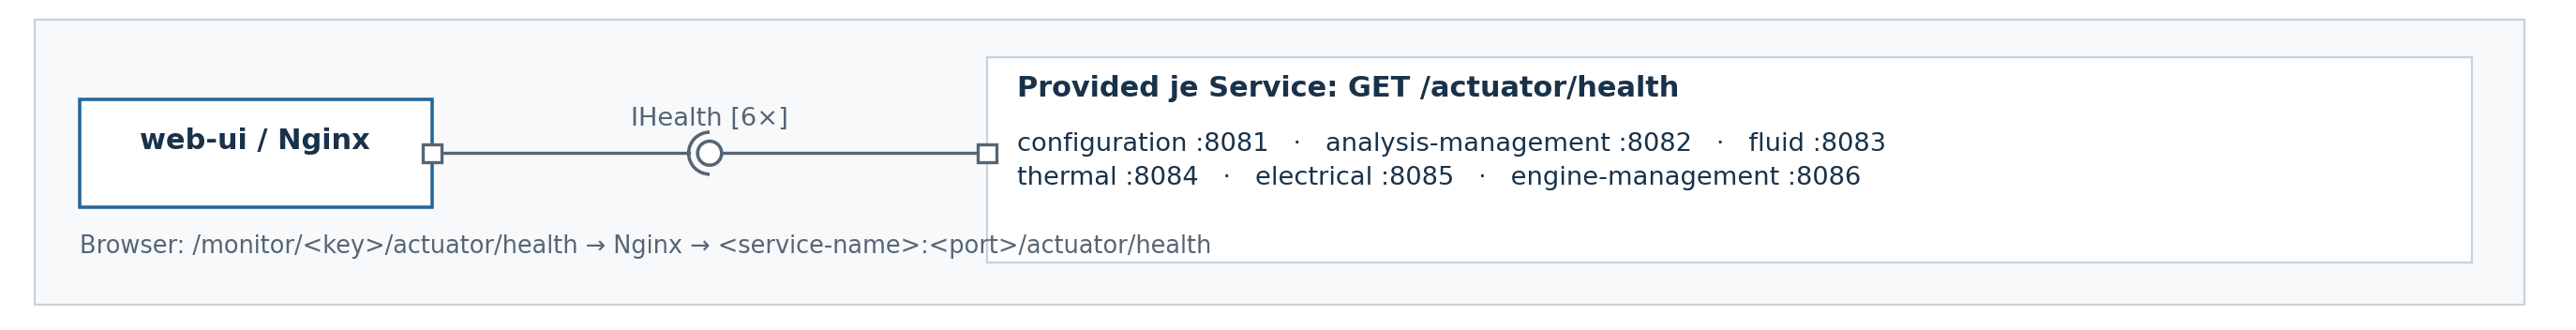
\includegraphics[width=\textwidth]{../diagrams/Bausteinsicht-monitoring.png}
  \caption{Bausteinsicht mit Monitoring-Sicht auf die laufenden Analysen.}
\end{figure}

\subsection{Qualitätsszenarien}
\begin{itemize}
  \item \textbf{Ausfall:} Thermal Analysis ist nicht erreichbar. Der Aufrufer bricht kontrolliert ab, markiert den Schritt als \code{FAILED} und die übrige Anwendung bleibt bedienbar.
  \item \textbf{Retry:} Nach Wiederherstellung wird nur der fehlgeschlagene Algorithmus erneut gestartet und die Kette anschlie\ss{}end fortgesetzt.
  \item \textbf{Nachvollziehbarkeit:} Zu jeder Analyse-ID sind Status und Resultate aller vier Algorithmen abrufbar.
  \item \textbf{Deployment:} Ein einzelner Analyse-Service kann unabhängig neu gebaut oder neu gestartet werden.
\end{itemize}

\newpage
